\documentclass{beamer}
\setbeamertemplate{navigation symbols}{}

\usepackage{amsmath}



\title[Collective SRL with ML]{Collective Semantic Role Labelling with Markov Logic}
\author[Riedel and Meza]{Sebastian Riedel \qquad Ivan Meza-Ruiz}
\institute[ICCS, UoE]{Institute for Communicating and Collaborative Systems\\
  School of Informatics\\
  University of Edinburgh, Scotland\\
  {\tt\{S.R.Riedel,I.V.Meza-Ruiz\}@sms.ed.ac.uk} }
\date{August, 2008}

\usetheme{Madrid}

\begin{document}
\begin{frame}
\titlepage
\end{frame}

\begin{frame}
    \frametitle{ Our intuitions of the SRL task}
    
    \begin{itemize}
        \item 
        \item A predicate can have at most one argument of a proper argument role.
    \end{itemize}
\end{frame}


\begin{frame}
    \frametitle{ Our intuitions of the SRL task}
    
    \begin{itemize}
        \item 
        \item Sense of a verbe correlates with the arguments roles of a verb.
    \end{itemize}
\end{frame}

\begin{frame}
    \frametitle{ Our intuitions of the SRL task}
    
    \begin{itemize}
        \item 
        \item Semantic role labels correlates with their POS tags
    \end{itemize}
\end{frame}

\begin{frame}
    \frametitle{Capturing our intuitions}
    
    \begin{itemize}
        \item Local: classifier, easy to do
        \item Global: pipeline, reranking, ILP, approximate heuristic search, harder to engineer
        \item Markov Logic (other, Statistical relational learning), easy to capture intuition
    \end{itemize}
\end{frame}

\begin{frame}
\tableofcontents
\end{frame}

\section{Markov Logic}

\begin{frame}
 \frametitle{Markov Logic}
 \begin{itemize}
 \item Combines of FOL and Markov Networks
 \item Defines a log-linear distribution over possible worlds
 \item Uses weigthed FOL formulae 
 \end{itemize}
\end{frame}

\section{Modelling}

\begin{frame}
    \frametitle{Vocabulary}
    \begin{itemize}
    \item Constants represents objects of the domain (Haag,VB,1,2,3,...)
    \item Predicates represent relations over the objects
    \end{itemize}

    There are two types: Observable and hidden. Some of the observable predicates are:
    \begin{itemize}
    \item \emph{word/2}, \emph{word(1,Haag)}
    \item \emph{pos/2},  \emph{pos(1,NNP)}
    \item \emph{path/3}, \emph{path(2,1,->)}
    \end{itemize}
    
\end{frame}

\begin{frame}
    \frametitle{Hidden predicates}
\begin{figure}
\begin{center}
   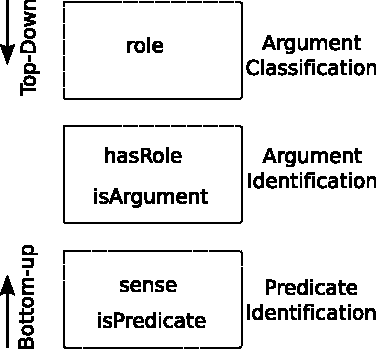
\includegraphics[scale=.70]{TaskArchitecture}
\end{center}
\caption{Hidden predicates}
\label{fig:task}
\end{figure}
\end{frame}

\begin{frame}
    \frametitle{Formulae}

%    A MLN is composed by the pairs ${(\phi,W)}$ where $\phi$ is FOL formulae and \emph{W} is a weight. 

    We use formulae to capture statements about the world. 
 \begin{eqnarray*}
a
 \end{eqnarray*}


\end{frame}


\begin{frame}
    \frametitle{Formulae}

%    A MLN is composed by the pairs ${(\phi,W)}$ where $\phi$ is FOL formulae and \emph{W} is a weight. 

    We use formulae to capture statements about the world. 
 \begin{eqnarray*}
a
 \end{eqnarray*}


\end{frame}


\begin{frame}
    \frametitle{Formulae}

%    A MLN is composed by the pairs ${(\phi,W)}$ where $\phi$ is FOL formulae and \emph{W} is a weight. 

    We use formulae to capture statements about the world. 
 \begin{eqnarray*}
a
 \end{eqnarray*}


\end{frame}


\begin{frame}
    \frametitle{Markov Logic Network}
    A set a weighted formulae is call an Markov Logic Network (MLN). 
    An MLN defines a Markov Network where:
    \begin{itemize}
    \item There is a binary node for each ground atom (e.g., \emph{role(2,1,A1)}.)
    \item There is a factor for each assignment of the free variable of each formulae. 
    \end{itemize}

%\begin{eqnarray*}
%\prob\left(\y\right)=\frac{1}{Z}\exp\left(
%\sum_{\left(\phi,w\right)\in M} w
%\sum_{\boldc\in C^{n_{\phi}}}f_{\boldc}^{\phi}\left(\y\right)
%\right)
%\end{eqnarray*}

\end{frame}


\begin{frame}
    \frametitle{Experiments}
    
\end{frame}



\end{document}
